\begin{figure}[H]
	\centering
	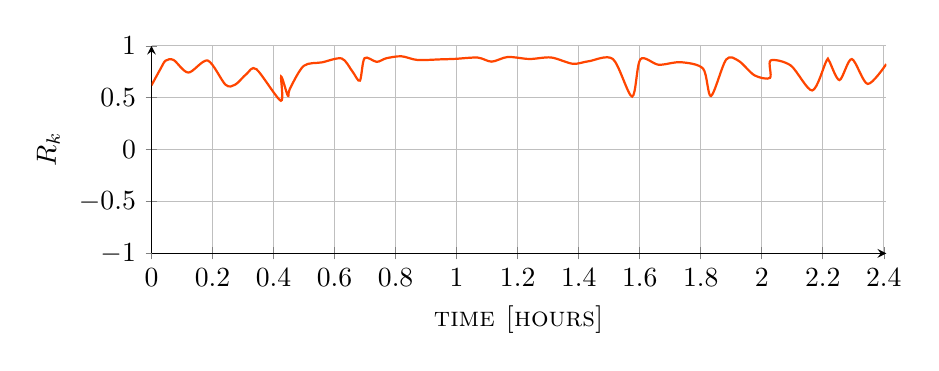
\begin{tikzpicture}
		\begin{axis}[xlabel=\textsc{time [hours]}, ylabel=\textsc{$R_k$}, axis lines=left, grid=major, width=0.9\linewidth, height=12em, ymax=1, ymin=-1]
			\addplot +[mark=none, OrangeRed, thick, smooth] table {
				0.0 0.6197258324124693
				0.029451666666666664 0.7780281900755717
				0.045969444444444445 0.8568861107993396
				0.07251972222222224 0.8631026530981518
				0.1207125 0.7420475867097251
				0.1844713888888889 0.8577557709343541
				0.24249166666666666 0.6252603862875922
				0.27450277777777776 0.6260366430947044
				0.3108925 0.7273702337589893
				0.34354944444444446 0.7752337667775194
				0.42398888888888886 0.4701261443944163
				0.4249991666666667 0.7028196005171105
				0.44684472222222227 0.5185459069092739
				0.45339027777777774 0.5858202814898343
				0.4986922222222222 0.8063907914235793
				0.5586986111111111 0.8406035293608265
				0.6233577777777778 0.8779896652803468
				0.6587488888888889 0.7512991803771675
				0.6829411111111111 0.6644443557745402
				0.6982236111111111 0.8813577541947395
				0.7379925 0.8452468641206403
				0.7694897222222222 0.8800279235961301
				0.8189947222222221 0.8990576196985542
				0.8714033333333334 0.8635864827719679
				0.9476627777777777 0.8695425662520067
				0.9957202777777777 0.8743194040956653
				1.069053888888889 0.8865111572192058
				1.1149888888888888 0.8475163642138497
				1.1675641666666665 0.8924012722543131
				1.2388225000000002 0.873011959272146
				1.3097197222222223 0.8875699734140305
				1.380589722222222 0.8268877009504354
				1.4330180555555554 0.8513901789111508
				1.5124180555555555 0.8719216321290916
				1.5751033333333335 0.5109562981582918
				1.6021605555555556 0.8704321775496318
				1.662174722222222 0.8175957565580481
				1.734423611111111 0.842191507641796
				1.807658888888889 0.7805109775548426
				1.8337208333333335 0.5160690570957521
				1.8833286111111112 0.8678191358901521
				1.9246980555555555 0.8542992991469915
				1.9763775 0.7152918607058433
				2.027149166666667 0.6914182838461037
				2.02891 0.8583944265847114
				2.0952330555555556 0.810100193534843
				2.165444722222222 0.5698351446078668
				2.211320277777778 0.850159971406908
				2.220778055555556 0.8539059120027274
				2.2547605555555554 0.6700373230774287
				2.2951580555555555 0.8725121926486323
				2.3471297222222223 0.6326024759580097
				2.4081411111111115 0.8241075262103797
			};
		\end{axis}
	\end{tikzpicture}
	\caption{Hyper-parameters optimization plot for the tool instance classifier based on random forest.}
	\label{fig:optimization_application_long_random_forest}
\end{figure}
\begin{table}[H]
	\centering
	\begin{tabular}{ll}
		\toprule
		\textsc{hyper-parameter} & \textsc{value}\\
		\midrule
		\verb|criterion| & entropy\\
		\verb|max_depth| & 20\\
		\verb|min_samples_leaf| & 6\\
		\verb|min_samples_split| & 18\\
		\verb|n_estimators| & 314\\
		\bottomrule
	\end{tabular}
	\caption{Optimal hyper-parameters for the tool instance classifier based on random forest.}
	\label{tab:hyperparameters_application_long_random_forest}
\end{table}
\begin{table}[H]
	\centering
	\begin{tabular}{lrrrr}
		\toprule
		\textsc{statistic} & \textsc{training set} & \textsc{dev set} & \textsc{kts} & \textsc{uts}\\
		\midrule
		samples & 955872 & 119484 & 119485 & 30144\\
		accuracy [$\%$] & 95.565 & 94.642 & 94.601 & 0.000\\
		balanced accuracy [$\%$] & 95.196 & 87.183 & 88.021 & 0.000\\
		precision [$\%$] & 79.996 & 74.641 & 75.061 & 0.000\\
		recall [$\%$] & 95.196 & 87.183 & 88.021 & 0.000\\
		Cohen’s kappa [$\%$] & 91.495 & 89.690 & 89.648 & 0.000\\
		F-score [$\%$] & 85.628 & 79.254 & 79.707 & 0.000\\
		Jaccard score [$\%$] & 76.831 & 68.057 & 68.871 & 0.000\\
		Hamming loss & 0.044 & 0.054 & 0.054 & 1.000\\
		zero-one loss & 0.044 & 0.054 & 0.054 & 1.000\\
		$R_k$ & 0.916 & 0.898 & 0.898 & 0.000\\
		\bottomrule
	\end{tabular}
	\caption{Classification statistics for the tool instance classifier based on random forest.}
	\label{tab:classification_application_long_random_forest}
\end{table}
\begin{table}[H]
	\centering
\resizebox{\linewidth}{!}{%
	\begin{tabular}{ll|llllllllllllllll}
	\setlength{\tabcolsep}{2pt}
		 & & \multicolumn{16}{c}{\textsc{inferred}}\\
		 & & \rotatebox{90}{\textsc{ch-48.0}} & \rotatebox{90}{\textsc{ch-68.0}} & \rotatebox{90}{\textsc{cu-7.55.1}} & \rotatebox{90}{\textsc{cu-7.61.0}} & \rotatebox{90}{\textsc{ed-42}} & \rotatebox{90}{\textsc{fi-42.0}} & \rotatebox{90}{\textsc{fi-62.0}} & \rotatebox{90}{\textsc{go-2.1}} & \rotatebox{90}{\textsc{ht-3.49.2}} & \rotatebox{90}{\textsc{hu-1.0}} & \rotatebox{90}{\textsc{ru-1.0.0}} & \rotatebox{90}{\textsc{sl-0.1.4}} & \rotatebox{90}{\textsc{sl-0.1.5}} & \rotatebox{90}{\textsc{wg-1.11.4}} & \rotatebox{90}{\textsc{wg-1.19.5}} & \rotatebox{90}{\textsc{wp-2.0.1}}\\
		\midrule
		\multirow{16}{*}{\rotatebox{90}{\textsc{target}}} & \textsc{ch-48.0} & 1128 & 80 & 14 & 4 & 91 & 18 & 20 & 61 & 4 & 4 & 0 & 0 & 3 & 3 & 10 & 10\\
		 & \textsc{ch-68.0} & 49 & 810 & 7 & 1 & 36 & 18 & 33 & 53 & 6 & 4 & 0 & 0 & 0 & 0 & 1 & 6\\
		 & \textsc{cu-7.55.1} & 0 & 1 & 150 & 6 & 0 & 0 & 3 & 4 & 5 & 0 & 0 & 0 & 1 & 2 & 0 & 0\\
		 & \textsc{cu-7.61.0} & 0 & 0 & 2 & 122 & 9 & 2 & 0 & 0 & 4 & 0 & 1 & 0 & 0 & 2 & 6 & 3\\
		 & \textsc{ed-42} & 75 & 37 & 2 & 21 & 2656 & 32 & 19 & 35 & 9 & 10 & 0 & 0 & 2 & 4 & 6 & 8\\
		 & \textsc{fi-42.0} & 26 & 22 & 9 & 2 & 41 & 646 & 51 & 34 & 12 & 5 & 2 & 0 & 2 & 4 & 3 & 10\\
		 & \textsc{fi-62.0} & 27 & 45 & 9 & 1 & 28 & 46 & 894 & 37 & 17 & 6 & 0 & 0 & 3 & 0 & 5 & 11\\
		 & \textsc{go-2.1} & 114 & 1191 & 50 & 2 & 157 & 74 & 320 & 74802 & 130 & 1459 & 93 & 4 & 5 & 18 & 10 & 265\\
		 & \textsc{ht-3.49.2} & 4 & 15 & 7 & 1 & 7 & 5 & 6 & 23 & 1224 & 2 & 0 & 0 & 1 & 0 & 0 & 3\\
		 & \textsc{hu-1.0} & 35 & 485 & 11 & 0 & 21 & 16 & 53 & 293 & 12 & 28435 & 18 & 0 & 3 & 6 & 0 & 53\\
		 & \textsc{ru-1.0.0} & 3 & 1 & 0 & 1 & 0 & 1 & 0 & 6 & 3 & 7 & 321 & 1 & 0 & 0 & 0 & 4\\
		 & \textsc{sl-0.1.4} & 0 & 0 & 0 & 0 & 0 & 0 & 0 & 0 & 0 & 0 & 1 & 607 & 6 & 0 & 0 & 0\\
		 & \textsc{sl-0.1.5} & 0 & 0 & 4 & 0 & 1 & 6 & 1 & 0 & 13 & 0 & 1 & 48 & 608 & 0 & 0 & 3\\
		 & \textsc{wg-1.11.4} & 2 & 1 & 1 & 2 & 4 & 3 & 0 & 8 & 0 & 1 & 1 & 0 & 0 & 259 & 0 & 1\\
		 & \textsc{wg-1.19.5} & 1 & 0 & 0 & 1 & 0 & 0 & 0 & 0 & 0 & 0 & 0 & 0 & 0 & 0 & 196 & 1\\
		 & \textsc{wp-2.0.1} & 1 & 5 & 1 & 5 & 4 & 4 & 2 & 6 & 3 & 1 & 0 & 0 & 1 & 3 & 0 & 176\\
	\end{tabular}
	}
	\caption{Confusion matrix for the tool instance classifier based on random forest on the KTS (where \textsc{go} = \textsc{goldeneye}, \textsc{fi} = \textsc{firefox}, \textsc{hu} = \textsc{hulk}, \textsc{wg} = \textsc{wget}, \textsc{ed} = \textsc{edge}, \textsc{ht} = \textsc{httrack}, \textsc{ch} = \textsc{chrome}, \textsc{ru} = \textsc{rudy}, \textsc{sl} = \textsc{slowloris}, \textsc{cu} = \textsc{curl} and \textsc{wp} = \textsc{wpull}.}
	\label{tab:confusion_application_long_random_forest}
\end{table}
\begin{figure}[H]
	\centering
	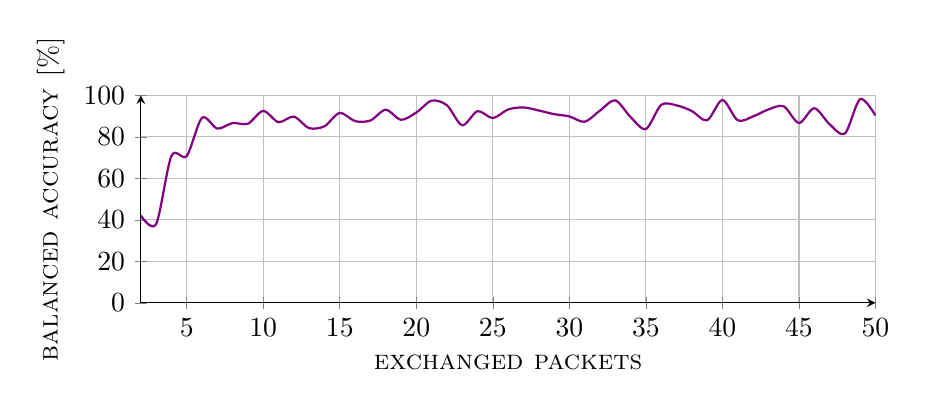
\begin{tikzpicture}
		\begin{axis}[xlabel=\textsc{exchanged packets}, ylabel=\textsc{balanced accuracy [$\%$]}, axis lines=left, grid=major, width=0.9\linewidth, height=12em, ymax=100, ymin=0]
			\addplot +[mark=none, Purple, thick, smooth] table {
				2.0 42.1317694310809
				3.0 37.878439412091915
				4.0 70.72245657277811
				5.0 70.71235573954769
				6.0 89.14889748864925
				7.0 83.96417829326143
				8.0 86.59482838733474
				9.0 86.31159671023984
				10.0 92.4514994816523
				11.0 87.04537601314483
				12.0 89.72490581780448
				13.0 84.17701401779034
				14.0 85.07621759697994
				15.0 91.53221571381057
				16.0 87.53223129389632
				17.0 87.83518209216757
				18.0 93.02528165082997
				19.0 88.20307786098297
				20.0 91.66526326760172
				21.0 97.39631353511471
				22.0 95.21231641921297
				23.0 85.54824154829835
				24.0 92.34650752105459
				25.0 89.00915582986988
				26.0 93.1776735772679
				27.0 94.15026864032708
				28.0 92.67009600897681
				29.0 90.9061436107292
				30.0 89.81332556332556
				31.0 87.2410628790297
				32.0 92.61959341255958
				33.0 97.55291005291005
				34.0 89.51820569703133
				35.0 83.73769748769749
				36.0 95.3997223583211
				37.0 95.14102059556605
				38.0 92.40216853853217
				39.0 87.93947539915281
				40.0 97.72727272727273
				41.0 87.93290043290042
				42.0 89.79166666666666
				43.0 93.14644499469402
				44.0 94.69696969696969
				45.0 86.6338924233661
				46.0 93.7610229276896
				47.0 86.06060606060606
				48.0 81.56043956043956
				49.0 98.18181818181819
				50.0 90.18253968253968
			};
		\end{axis}
	\end{tikzpicture}
	\caption{Balanced accuracy vs. exchange packets plot for the tool instance classifier based on random forest on the KTS.}
	\label{fig:packets_application_long_random_forest}
\end{figure}
\begin{table}[H]
	\centering
	\begin{subtable}{.45\linewidth}
		\centering
	\begin{tabular}{ll}
		\toprule
		\textsc{inferred class} & \textsc{samples}\\
		\midrule
		chrome-48.0.2564.109 & 367\\
		chrome-68.0.3440.84 & 226\\
		curl-7.55.1 & 9\\
		edge-42.17134.1.0 & 356\\
		firefox-42.0 & 607\\
		firefox-62.0 & 1805\\
		goldeneye-2.1 & 377\\
		httrack-3.49.2 & 47\\
		hulk-1.0 & 49\\
		rudy-1.0.0 & 33\\
		slowloris-0.1.5 & 52\\
		wget-1.19.5 & 60\\
		wpull-2.0.1 & 2546\\
		\bottomrule
	\end{tabular}
	\caption{Classification of \textsc{firefox-68.0}.}
	\end{subtable}
	\begin{subtable}{.45\linewidth}
		\centering
	\begin{tabular}{ll}
		\toprule
		\textsc{inferred class} & \textsc{samples}\\
		\midrule
		chrome-48.0.2564.109 & 112\\
		chrome-68.0.3440.84 & 168\\
		curl-7.55.1 & 53\\
		curl-7.61.0 & 2\\
		edge-42.17134.1.0 & 260\\
		firefox-42.0 & 224\\
		firefox-62.0 & 296\\
		goldeneye-2.1 & 1579\\
		httrack-3.49.2 & 164\\
		hulk-1.0 & 223\\
		rudy-1.0.0 & 25\\
		slowloris-0.1.5 & 11\\
		wget-1.11.4 & 84\\
		wget-1.19.5 & 23\\
		wpull-2.0.1 & 441\\
		\bottomrule
	\end{tabular}
	\caption{Classification of \textsc{grabsite-2.1.16}.}
	\end{subtable}
	\begin{subtable}{.45\linewidth}
		\centering
	\begin{tabular}{ll}
		\toprule
		\textsc{inferred class} & \textsc{samples}\\
		\midrule
		chrome-48.0.2564.109 & 2365\\
		chrome-68.0.3440.84 & 2178\\
		curl-7.55.1 & 103\\
		curl-7.61.0 & 5\\
		edge-42.17134.1.0 & 382\\
		firefox-42.0 & 275\\
		firefox-62.0 & 714\\
		goldeneye-2.1 & 2431\\
		httrack-3.49.2 & 231\\
		hulk-1.0 & 35\\
		rudy-1.0.0 & 18\\
		slowloris-0.1.5 & 6\\
		wget-1.11.4 & 12\\
		wget-1.19.5 & 5\\
		wpull-2.0.1 & 190\\
		\bottomrule
	\end{tabular}
	\caption{Classification of \textsc{opera-62.0.3331.66}.}
	\end{subtable}
	\begin{subtable}{.45\linewidth}
		\centering
	\begin{tabular}{ll}
		\toprule
		\textsc{inferred class} & \textsc{samples}\\
		\midrule
		chrome-48.0.2564.109 & 165\\
		chrome-68.0.3440.84 & 27\\
		curl-7.55.1 & 78\\
		curl-7.61.0 & 22\\
		edge-42.17134.1.0 & 1795\\
		firefox-42.0 & 394\\
		firefox-62.0 & 1220\\
		goldeneye-2.1 & 1212\\
		httrack-3.49.2 & 341\\
		hulk-1.0 & 33\\
		rudy-1.0.0 & 4061\\
		slowloris-0.1.4 & 1\\
		slowloris-0.1.5 & 56\\
		wget-1.11.4 & 25\\
		wget-1.19.5 & 8\\
		wpull-2.0.1 & 1557\\
		\bottomrule
	\end{tabular}
	\caption{Classification of \textsc{slowhttptest-1.6}.}
	\end{subtable}
	\caption{Classification of unknown tools for the tool instance classifier based on random forest.}
	\label{tab:unknown_application_long_random_forest}
\end{table}
